\documentclass[1p]{elsarticle_modified}
%\bibliographystyle{elsarticle-num}

%\usepackage[colorlinks]{hyperref}
%\usepackage{abbrmath_seonhwa} %\Abb, \Ascr, \Acal ,\Abf, \Afrak
\usepackage{amsfonts}
\usepackage{amssymb}
\usepackage{amsmath}
\usepackage{amsthm}
\usepackage{scalefnt}
\usepackage{amsbsy}
\usepackage{kotex}
\usepackage{caption}
\usepackage{subfig}
\usepackage{color}
\usepackage{graphicx}
\usepackage{xcolor} %% white, black, red, green, blue, cyan, magenta, yellow
\usepackage{float}
\usepackage{setspace}
\usepackage{hyperref}

\usepackage{tikz}
\usetikzlibrary{arrows}

\usepackage{multirow}
\usepackage{array} % fixed length table
\usepackage{hhline}

%%%%%%%%%%%%%%%%%%%%%
\makeatletter
\renewcommand*\env@matrix[1][\arraystretch]{%
	\edef\arraystretch{#1}%
	\hskip -\arraycolsep
	\let\@ifnextchar\new@ifnextchar
	\array{*\c@MaxMatrixCols c}}
\makeatother %https://tex.stackexchange.com/questions/14071/how-can-i-increase-the-line-spacing-in-a-matrix
%%%%%%%%%%%%%%%

\usepackage[normalem]{ulem}

\newcommand{\msout}[1]{\ifmmode\text{\sout{\ensuremath{#1}}}\else\sout{#1}\fi}
%SOURCE: \msout is \stkout macro in https://tex.stackexchange.com/questions/20609/strikeout-in-math-mode

\newcommand{\cancel}[1]{
	\ifmmode
	{\color{red}\msout{#1}}
	\else
	{\color{red}\sout{#1}}
	\fi
}

\newcommand{\add}[1]{
	{\color{blue}\uwave{#1}}
}

\newcommand{\replace}[2]{
	\ifmmode
	{\color{red}\msout{#1}}{\color{blue}\uwave{#2}}
	\else
	{\color{red}\sout{#1}}{\color{blue}\uwave{#2}}
	\fi
}

\newcommand{\Sol}{\mathcal{S}} %segment
\newcommand{\D}{D} %diagram
\newcommand{\A}{\mathcal{A}} %arc


%%%%%%%%%%%%%%%%%%%%%%%%%%%%%5 test

\def\sl{\operatorname{\textup{SL}}(2,\Cbb)}
\def\psl{\operatorname{\textup{PSL}}(2,\Cbb)}
\def\quan{\mkern 1mu \triangleright \mkern 1mu}

\theoremstyle{definition}
\newtheorem{thm}{Theorem}[section]
\newtheorem{prop}[thm]{Proposition}
\newtheorem{lem}[thm]{Lemma}
\newtheorem{ques}[thm]{Question}
\newtheorem{cor}[thm]{Corollary}
\newtheorem{defn}[thm]{Definition}
\newtheorem{exam}[thm]{Example}
\newtheorem{rmk}[thm]{Remark}
\newtheorem{alg}[thm]{Algorithm}

\newcommand{\I}{\sqrt{-1}}
\begin{document}

%\begin{frontmatter}
%
%\title{Boundary parabolic representations of knots up to 8 crossings}
%
%%% Group authors per affiliation:
%\author{Yunhi Cho} 
%\address{Department of Mathematics, University of Seoul, Seoul, Korea}
%\ead{yhcho@uos.ac.kr}
%
%
%\author{Seonhwa Kim} %\fnref{s_kim}}
%\address{Center for Geometry and Physics, Institute for Basic Science, Pohang, 37673, Korea}
%\ead{ryeona17@ibs.re.kr}
%
%\author{Hyuk Kim}
%\address{Department of Mathematical Sciences, Seoul National University, Seoul 08826, Korea}
%\ead{hyukkim@snu.ac.kr}
%
%\author{Seokbeom Yoon}
%\address{Department of Mathematical Sciences, Seoul National University, Seoul, 08826,  Korea}
%\ead{sbyoon15@snu.ac.kr}
%
%\begin{abstract}
%We find all boundary parabolic representation of knots up to 8 crossings.
%
%\end{abstract}
%\begin{keyword}
%    \MSC[2010] 57M25 
%\end{keyword}
%
%\end{frontmatter}

%\linenumbers
%\tableofcontents
%
\newcommand\colored[1]{\textcolor{white}{\rule[-0.35ex]{0.8em}{1.4ex}}\kern-0.8em\color{red} #1}%
%\newcommand\colored[1]{\textcolor{white}{ #1}\kern-2.17ex	\textcolor{white}{ #1}\kern-1.81ex	\textcolor{white}{ #1}\kern-2.15ex\color{red}#1	}

{\Large $\underline{12a_{0280}~(K12a_{0280})}$}

\setlength{\tabcolsep}{10pt}
\renewcommand{\arraystretch}{1.6}
\vspace{1cm}\begin{tabular}{m{100pt}>{\centering\arraybackslash}m{274pt}}
\multirow{5}{120pt}{
	\centering
	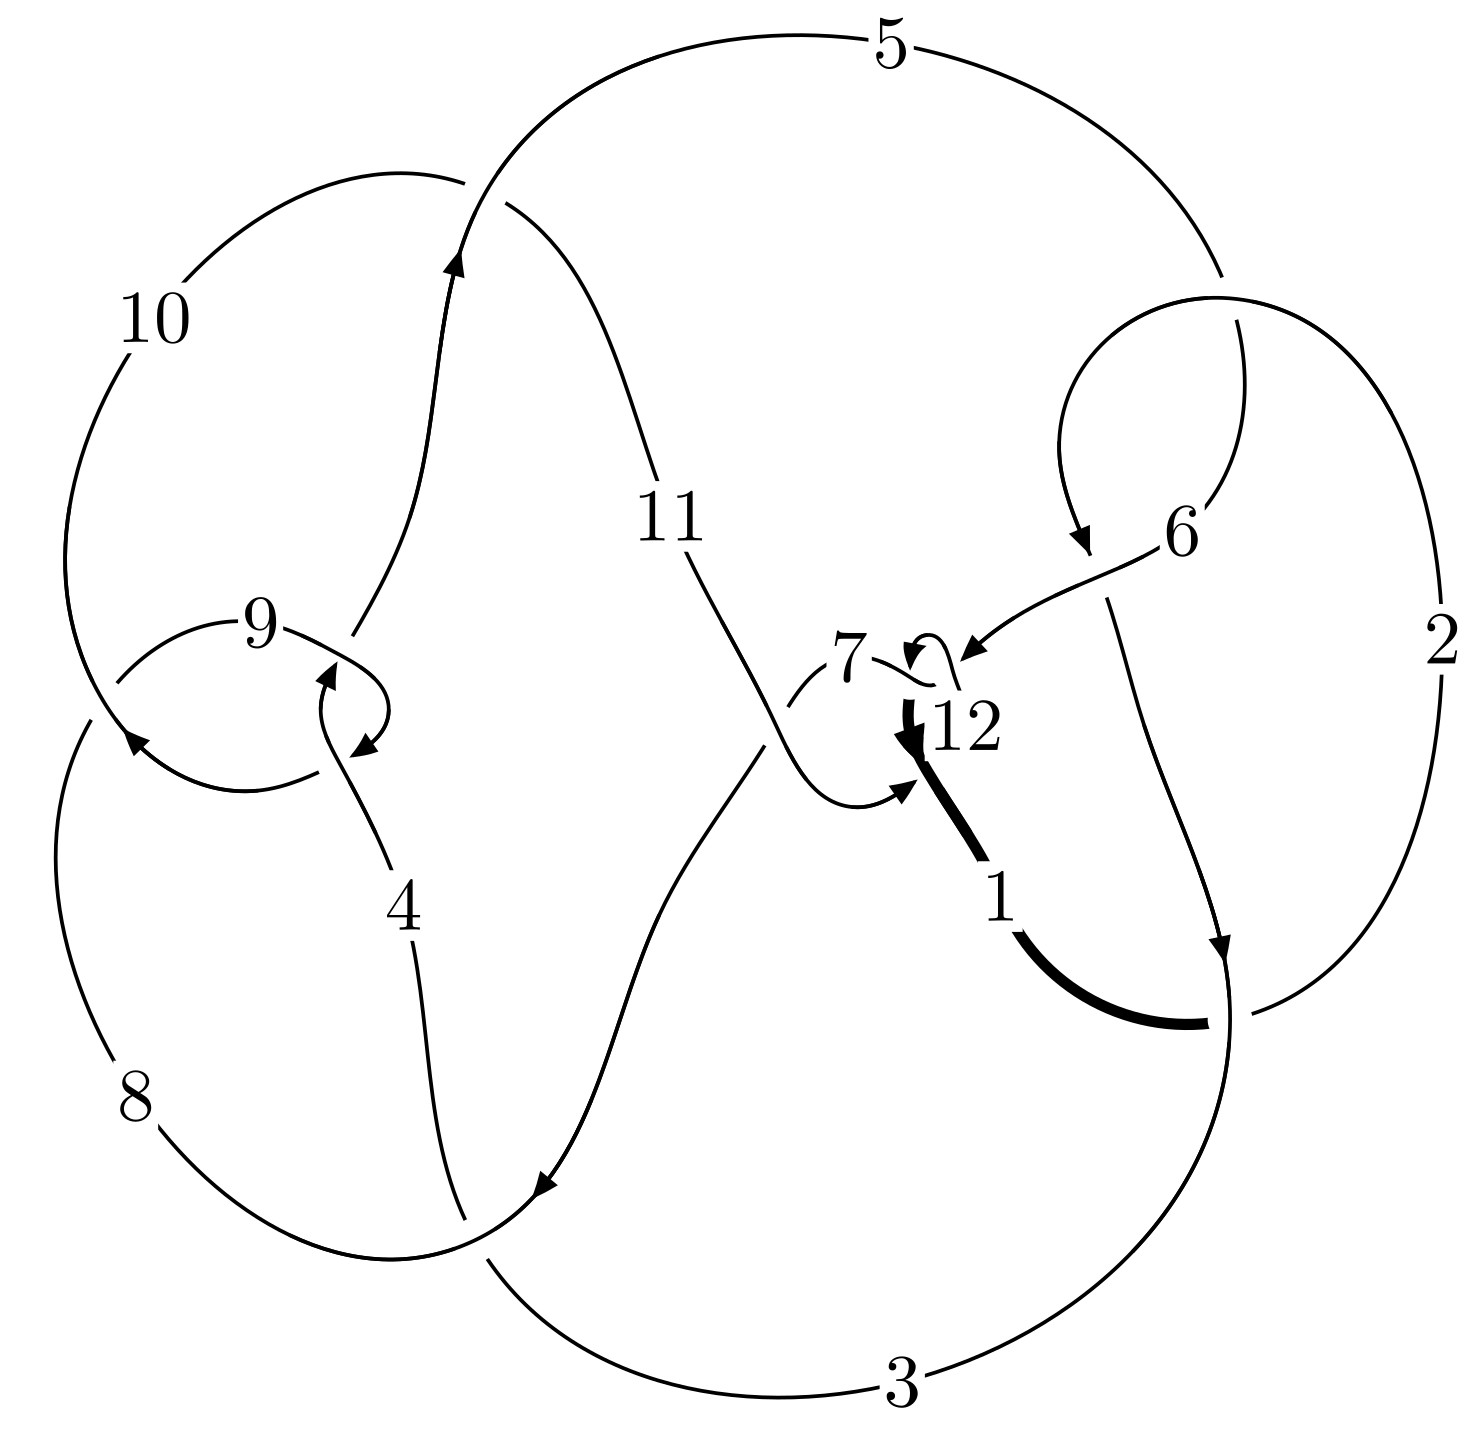
\includegraphics[width=112pt]{../../../GIT/diagram.site/Diagrams/png/1081_12a_0280.png}\\
\ \ \ A knot diagram\footnotemark}&
\allowdisplaybreaks
\textbf{Linearized knot diagam} \\
\cline{2-2}
 &
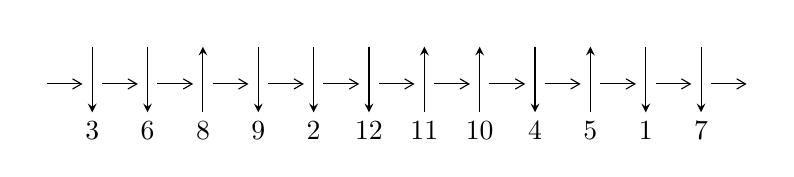
\begin{tikzpicture}[x=20pt, y=17pt]
	% nodes
	\node (C0) at (0, 0) {};
	\node (C1) at (1, 0) {};
	\node (C1U) at (1, +1) {};
	\node (C1D) at (1, -1) {3};

	\node (C2) at (2, 0) {};
	\node (C2U) at (2, +1) {};
	\node (C2D) at (2, -1) {6};

	\node (C3) at (3, 0) {};
	\node (C3U) at (3, +1) {};
	\node (C3D) at (3, -1) {8};

	\node (C4) at (4, 0) {};
	\node (C4U) at (4, +1) {};
	\node (C4D) at (4, -1) {9};

	\node (C5) at (5, 0) {};
	\node (C5U) at (5, +1) {};
	\node (C5D) at (5, -1) {2};

	\node (C6) at (6, 0) {};
	\node (C6U) at (6, +1) {};
	\node (C6D) at (6, -1) {12};

	\node (C7) at (7, 0) {};
	\node (C7U) at (7, +1) {};
	\node (C7D) at (7, -1) {11};

	\node (C8) at (8, 0) {};
	\node (C8U) at (8, +1) {};
	\node (C8D) at (8, -1) {10};

	\node (C9) at (9, 0) {};
	\node (C9U) at (9, +1) {};
	\node (C9D) at (9, -1) {4};

	\node (C10) at (10, 0) {};
	\node (C10U) at (10, +1) {};
	\node (C10D) at (10, -1) {5};

	\node (C11) at (11, 0) {};
	\node (C11U) at (11, +1) {};
	\node (C11D) at (11, -1) {1};

	\node (C12) at (12, 0) {};
	\node (C12U) at (12, +1) {};
	\node (C12D) at (12, -1) {7};
	\node (C13) at (13, 0) {};

	% arrows
	\draw[->,>={angle 60}]
	(C0) edge (C1) (C1) edge (C2) (C2) edge (C3) (C3) edge (C4) (C4) edge (C5) (C5) edge (C6) (C6) edge (C7) (C7) edge (C8) (C8) edge (C9) (C9) edge (C10) (C10) edge (C11) (C11) edge (C12) (C12) edge (C13) ;	\draw[->,>=stealth]
	(C1U) edge (C1D) (C2U) edge (C2D) (C3D) edge (C3U) (C4U) edge (C4D) (C5U) edge (C5D) (C6U) edge (C6D) (C7D) edge (C7U) (C8D) edge (C8U) (C9U) edge (C9D) (C10D) edge (C10U) (C11U) edge (C11D) (C12U) edge (C12D) ;
	\end{tikzpicture} \\
\hhline{~~} \\& 
\textbf{Solving Sequence} \\ \cline{2-2} 
 &
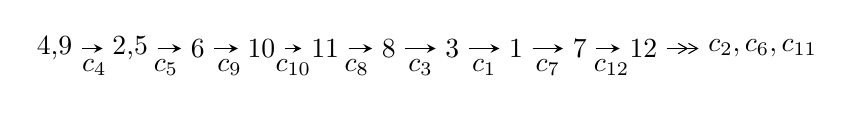
\begin{tikzpicture}[x=23pt, y=7pt]
	% node
	\node (A0) at (-1/8, 0) {4,9};
	\node (A1) at (17/16, 0) {2,5};
	\node (A2) at (17/8, 0) {6};
	\node (A3) at (25/8, 0) {10};
	\node (A4) at (33/8, 0) {11};
	\node (A5) at (41/8, 0) {8};
	\node (A6) at (49/8, 0) {3};
	\node (A7) at (57/8, 0) {1};
	\node (A8) at (65/8, 0) {7};
	\node (A9) at (73/8, 0) {12};
	\node (C1) at (1/2, -1) {$c_{4}$};
	\node (C2) at (13/8, -1) {$c_{5}$};
	\node (C3) at (21/8, -1) {$c_{9}$};
	\node (C4) at (29/8, -1) {$c_{10}$};
	\node (C5) at (37/8, -1) {$c_{8}$};
	\node (C6) at (45/8, -1) {$c_{3}$};
	\node (C7) at (53/8, -1) {$c_{1}$};
	\node (C8) at (61/8, -1) {$c_{7}$};
	\node (C9) at (69/8, -1) {$c_{12}$};
	\node (A10) at (11, 0) {$c_{2},c_{6},c_{11}$};

	% edge
	\draw[->,>=stealth]	
	(A0) edge (A1) (A1) edge (A2) (A2) edge (A3) (A3) edge (A4) (A4) edge (A5) (A5) edge (A6) (A6) edge (A7) (A7) edge (A8) (A8) edge (A9) ;
	\draw[->>,>={angle 60}]	
	(A9) edge (A10);
\end{tikzpicture} \\ 

\end{tabular} \\

\footnotetext{
The image of knot diagram is generated by the software ``\textbf{Draw programme}" developed by Andrew Bartholomew(\url{http://www.layer8.co.uk/maths/draw/index.htm\#Running-draw}), where we modified some parts for our purpose(\url{https://github.com/CATsTAILs/LinksPainter}).
}\phantom \\ \newline 
\centering \textbf{Ideals for irreducible components\footnotemark of $X_{\text{par}}$} 
 
\begin{align*}
I^u_{1}&=\langle 
- u^{38}+3 u^{37}+\cdots+b-3,\;3 u^{39}-7 u^{38}+\cdots+2 a-4,\;u^{40}-3 u^{39}+\cdots-6 u+2\rangle \\
I^u_{2}&=\langle 
205 u^{31} a-187 u^{31}+\cdots-343 a+410,\;- u^{31}-2 u^{30}+\cdots-4 a+4,\;u^{32}+u^{31}+\cdots-2 u-1\rangle \\
I^u_{3}&=\langle 
- u^3+u^2+b- u+1,\;u^3-2 u^2+2 a-2,\;u^4+2 u^2+2\rangle \\
\\
I^v_{1}&=\langle 
a,\;b+1,\;v+1\rangle \\
\end{align*}
\raggedright * 4 irreducible components of $\dim_{\mathbb{C}}=0$, with total 109 representations.\\
\footnotetext{All coefficients of polynomials are rational numbers. But the coefficients are sometimes approximated in decimal forms when there is not enough margin.}
\newpage
\renewcommand{\arraystretch}{1}
\centering \section*{I. $I^u_{1}= \langle - u^{38}+3 u^{37}+\cdots+b-3,\;3 u^{39}-7 u^{38}+\cdots+2 a-4,\;u^{40}-3 u^{39}+\cdots-6 u+2 \rangle$}
\flushleft \textbf{(i) Arc colorings}\\
\begin{tabular}{m{7pt} m{180pt} m{7pt} m{180pt} }
\flushright $a_{4}=$&$\begin{pmatrix}1\\0\end{pmatrix}$ \\
\flushright $a_{9}=$&$\begin{pmatrix}0\\u\end{pmatrix}$ \\
\flushright $a_{2}=$&$\begin{pmatrix}-\frac{3}{2} u^{39}+\frac{7}{2} u^{38}+\cdots-4 u+2\\u^{38}-3 u^{37}+\cdots-5 u+3\end{pmatrix}$ \\
\flushright $a_{5}=$&$\begin{pmatrix}1\\u^2\end{pmatrix}$ \\
\flushright $a_{6}=$&$\begin{pmatrix}-\frac{1}{2} u^{39}+\frac{3}{2} u^{38}+\cdots-4 u+3\\- u^{38}+2 u^{37}+\cdots+3 u-1\end{pmatrix}$ \\
\flushright $a_{10}=$&$\begin{pmatrix}- u\\u\end{pmatrix}$ \\
\flushright $a_{11}=$&$\begin{pmatrix}u^3\\u^5+u^3+u\end{pmatrix}$ \\
\flushright $a_{8}=$&$\begin{pmatrix}- u^3\\u^3+u\end{pmatrix}$ \\
\flushright $a_{3}=$&$\begin{pmatrix}- u^6- u^4+1\\u^6+2 u^4+u^2\end{pmatrix}$ \\
\flushright $a_{1}=$&$\begin{pmatrix}-\frac{7}{2} u^{39}+\frac{17}{2} u^{38}+\cdots-10 u+3\\2 u^{38}-7 u^{37}+\cdots-11 u+7\end{pmatrix}$ \\
\flushright $a_{7}=$&$\begin{pmatrix}- u^{11}-2 u^9-2 u^7- u^3\\- u^{13}-3 u^{11}-5 u^9-4 u^7-2 u^5+u^3+u\end{pmatrix}$ \\
\flushright $a_{12}=$&$\begin{pmatrix}\frac{3}{2} u^{39}-\frac{7}{2} u^{38}+\cdots+4 u-1\\- u^{38}+3 u^{37}+\cdots+6 u-3\end{pmatrix}$\\&\end{tabular}
\flushleft \textbf{(ii) Obstruction class $= -1$}\\~\\
\flushleft \textbf{(iii) Cusp Shapes $= 2 u^{39}-6 u^{38}+20 u^{37}-54 u^{36}+90 u^{35}-238 u^{34}+238 u^{33}-648 u^{32}+384 u^{31}-1158 u^{30}+312 u^{29}-1278 u^{28}-154 u^{27}-492 u^{26}-898 u^{25}+1018 u^{24}-1550 u^{23}+2192 u^{22}-1746 u^{21}+2064 u^{20}-1346 u^{19}+876 u^{18}-498 u^{17}-254 u^{16}+320 u^{15}-624 u^{14}+616 u^{13}-464 u^{12}+388 u^{11}-200 u^{10}+68 u^9-16 u^8-38 u^7+56 u^6-38 u^5+40 u^4-30 u^3+8 u^2-14 u+8$}\\~\\
\newpage\renewcommand{\arraystretch}{1}
\flushleft \textbf{(iv) u-Polynomials at the component}\newline \\
\begin{tabular}{m{50pt}|m{274pt}}
Crossings & \hspace{64pt}u-Polynomials at each crossing \\
\hline $$\begin{aligned}c_{1},c_{11}\end{aligned}$$&$\begin{aligned}
&u^{40}+19 u^{39}+\cdots+8 u+1
\end{aligned}$\\
\hline $$\begin{aligned}c_{2},c_{5},c_{6}\\c_{12}\end{aligned}$$&$\begin{aligned}
&u^{40}+u^{39}+\cdots-4 u^2+1
\end{aligned}$\\
\hline $$\begin{aligned}c_{3},c_{10}\end{aligned}$$&$\begin{aligned}
&u^{40}+3 u^{39}+\cdots+62 u+2
\end{aligned}$\\
\hline $$\begin{aligned}c_{4},c_{9}\end{aligned}$$&$\begin{aligned}
&u^{40}-3 u^{39}+\cdots-6 u+2
\end{aligned}$\\
\hline $$\begin{aligned}c_{7}\end{aligned}$$&$\begin{aligned}
&u^{40}+3 u^{39}+\cdots-256 u+256
\end{aligned}$\\
\hline $$\begin{aligned}c_{8}\end{aligned}$$&$\begin{aligned}
&u^{40}-21 u^{39}+\cdots-4 u+4
\end{aligned}$\\
\hline
\end{tabular}\\~\\
\newpage\renewcommand{\arraystretch}{1}
\flushleft \textbf{(v) Riley Polynomials at the component}\newline \\
\begin{tabular}{m{50pt}|m{274pt}}
Crossings & \hspace{64pt}Riley Polynomials at each crossing \\
\hline $$\begin{aligned}c_{1},c_{11}\end{aligned}$$&$\begin{aligned}
&y^{40}+13 y^{39}+\cdots-8 y+1
\end{aligned}$\\
\hline $$\begin{aligned}c_{2},c_{5},c_{6}\\c_{12}\end{aligned}$$&$\begin{aligned}
&y^{40}-19 y^{39}+\cdots-8 y+1
\end{aligned}$\\
\hline $$\begin{aligned}c_{3},c_{10}\end{aligned}$$&$\begin{aligned}
&y^{40}-27 y^{39}+\cdots-1244 y+4
\end{aligned}$\\
\hline $$\begin{aligned}c_{4},c_{9}\end{aligned}$$&$\begin{aligned}
&y^{40}+21 y^{39}+\cdots+4 y+4
\end{aligned}$\\
\hline $$\begin{aligned}c_{7}\end{aligned}$$&$\begin{aligned}
&y^{40}+17 y^{39}+\cdots-1441792 y+65536
\end{aligned}$\\
\hline $$\begin{aligned}c_{8}\end{aligned}$$&$\begin{aligned}
&y^{40}-3 y^{39}+\cdots+80 y+16
\end{aligned}$\\
\hline
\end{tabular}\\~\\
\newpage\flushleft \textbf{(vi) Complex Volumes and Cusp Shapes}
$$\begin{array}{c|c|c}  
\text{Solutions to }I^u_{1}& \I (\text{vol} + \sqrt{-1}CS) & \text{Cusp shape}\\
 \hline 
\begin{aligned}
u &= \phantom{-}0.032066 + 0.987972 I \\
a &= \phantom{-}0.79918 - 1.21680 I \\
b &= -0.098470 + 0.680905 I\end{aligned}
 & \phantom{-}2.63292 + 1.38793 I & \phantom{-}3.69460 - 3.72098 I \\ \hline\begin{aligned}
u &= \phantom{-}0.032066 - 0.987972 I \\
a &= \phantom{-}0.79918 + 1.21680 I \\
b &= -0.098470 - 0.680905 I\end{aligned}
 & \phantom{-}2.63292 - 1.38793 I & \phantom{-}3.69460 + 3.72098 I \\ \hline\begin{aligned}
u &= -0.603533 + 0.828822 I \\
a &= -1.69497 - 1.57214 I \\
b &= \phantom{-}0.15771 + 1.68881 I\end{aligned}
 & -6.26949 + 10.98300 I & -9.24065 - 9.80825 I \\ \hline\begin{aligned}
u &= -0.603533 - 0.828822 I \\
a &= -1.69497 + 1.57214 I \\
b &= \phantom{-}0.15771 - 1.68881 I\end{aligned}
 & -6.26949 - 10.98300 I & -9.24065 + 9.80825 I \\ \hline\begin{aligned}
u &= -0.621730 + 0.712285 I \\
a &= \phantom{-}1.139040 + 0.396240 I \\
b &= -0.95556 - 1.55078 I\end{aligned}
 & -6.60486 - 6.20651 I & -10.15571 + 3.67210 I \\ \hline\begin{aligned}
u &= -0.621730 - 0.712285 I \\
a &= \phantom{-}1.139040 - 0.396240 I \\
b &= -0.95556 + 1.55078 I\end{aligned}
 & -6.60486 + 6.20651 I & -10.15571 - 3.67210 I \\ \hline\begin{aligned}
u &= -0.481507 + 0.789783 I \\
a &= \phantom{-}0.648708 + 0.018988 I \\
b &= -0.141348 + 0.130562 I\end{aligned}
 & -0.36391 + 1.99287 I & -2.40004 - 3.73815 I \\ \hline\begin{aligned}
u &= -0.481507 - 0.789783 I \\
a &= \phantom{-}0.648708 - 0.018988 I \\
b &= -0.141348 - 0.130562 I\end{aligned}
 & -0.36391 - 1.99287 I & -2.40004 + 3.73815 I \\ \hline\begin{aligned}
u &= \phantom{-}0.491208 + 0.978630 I \\
a &= -0.81937 + 1.39099 I \\
b &= \phantom{-}0.109214 - 1.360820 I\end{aligned}
 & -0.16272 - 6.27605 I & -4.06803 + 10.74221 I \\ \hline\begin{aligned}
u &= \phantom{-}0.491208 - 0.978630 I \\
a &= -0.81937 - 1.39099 I \\
b &= \phantom{-}0.109214 + 1.360820 I\end{aligned}
 & -0.16272 + 6.27605 I & -4.06803 - 10.74221 I\\
 \hline 
 \end{array}$$\newpage$$\begin{array}{c|c|c}  
\text{Solutions to }I^u_{1}& \I (\text{vol} + \sqrt{-1}CS) & \text{Cusp shape}\\
 \hline 
\begin{aligned}
u &= \phantom{-}0.231511 + 1.113940 I \\
a &= \phantom{-}0.38329 + 1.48578 I \\
b &= -0.133956 - 1.058470 I\end{aligned}
 & -0.38661 - 7.27037 I & -2.50119 + 7.55106 I \\ \hline\begin{aligned}
u &= \phantom{-}0.231511 - 1.113940 I \\
a &= \phantom{-}0.38329 - 1.48578 I \\
b &= -0.133956 + 1.058470 I\end{aligned}
 & -0.38661 + 7.27037 I & -2.50119 - 7.55106 I \\ \hline\begin{aligned}
u &= \phantom{-}0.810351 + 0.193335 I \\
a &= -1.06622 - 1.29812 I \\
b &= \phantom{-}0.94040 - 1.69712 I\end{aligned}
 & -3.06749 + 12.23140 I & -7.51087 - 7.91346 I \\ \hline\begin{aligned}
u &= \phantom{-}0.810351 - 0.193335 I \\
a &= -1.06622 + 1.29812 I \\
b &= \phantom{-}0.94040 + 1.69712 I\end{aligned}
 & -3.06749 - 12.23140 I & -7.51087 + 7.91346 I \\ \hline\begin{aligned}
u &= -0.482698 + 1.065100 I \\
a &= -0.201840 - 0.655189 I \\
b &= \phantom{-}0.187841 + 0.901163 I\end{aligned}
 & \phantom{-}0.58711 + 3.31811 I & -0.88906 - 1.84785 I \\ \hline\begin{aligned}
u &= -0.482698 - 1.065100 I \\
a &= -0.201840 + 0.655189 I \\
b &= \phantom{-}0.187841 - 0.901163 I\end{aligned}
 & \phantom{-}0.58711 - 3.31811 I & -0.88906 + 1.84785 I \\ \hline\begin{aligned}
u &= \phantom{-}0.735874 + 0.291866 I \\
a &= \phantom{-}1.005670 + 0.058018 I \\
b &= -0.688345 - 0.001466 I\end{aligned}
 & -4.71000 - 4.49018 I & -9.32153 + 4.94666 I \\ \hline\begin{aligned}
u &= \phantom{-}0.735874 - 0.291866 I \\
a &= \phantom{-}1.005670 - 0.058018 I \\
b &= -0.688345 + 0.001466 I\end{aligned}
 & -4.71000 + 4.49018 I & -9.32153 - 4.94666 I \\ \hline\begin{aligned}
u &= -0.789239 + 0.057041 I \\
a &= -0.060699 + 1.159700 I \\
b &= \phantom{-}0.92550 + 1.37773 I\end{aligned}
 & \phantom{-}3.56585 - 5.08226 I & -1.98598 + 6.14285 I \\ \hline\begin{aligned}
u &= -0.789239 - 0.057041 I \\
a &= -0.060699 - 1.159700 I \\
b &= \phantom{-}0.92550 - 1.37773 I\end{aligned}
 & \phantom{-}3.56585 + 5.08226 I & -1.98598 - 6.14285 I\\
 \hline 
 \end{array}$$\newpage$$\begin{array}{c|c|c}  
\text{Solutions to }I^u_{1}& \I (\text{vol} + \sqrt{-1}CS) & \text{Cusp shape}\\
 \hline 
\begin{aligned}
u &= \phantom{-}0.762371 + 0.132104 I \\
a &= \phantom{-}0.507160 + 0.391032 I \\
b &= \phantom{-}0.517802 + 1.069740 I\end{aligned}
 & \phantom{-}2.25804 + 2.12425 I & -0.766744 - 0.783432 I \\ \hline\begin{aligned}
u &= \phantom{-}0.762371 - 0.132104 I \\
a &= \phantom{-}0.507160 - 0.391032 I \\
b &= \phantom{-}0.517802 - 1.069740 I\end{aligned}
 & \phantom{-}2.25804 - 2.12425 I & -0.766744 + 0.783432 I \\ \hline\begin{aligned}
u &= \phantom{-}0.538422 + 1.126370 I \\
a &= \phantom{-}0.287354 + 0.772248 I \\
b &= -0.106299 - 0.840485 I\end{aligned}
 & -2.27245 - 0.32612 I & -6.24945 - 1.38108 I \\ \hline\begin{aligned}
u &= \phantom{-}0.538422 - 1.126370 I \\
a &= \phantom{-}0.287354 - 0.772248 I \\
b &= -0.106299 + 0.840485 I\end{aligned}
 & -2.27245 + 0.32612 I & -6.24945 + 1.38108 I \\ \hline\begin{aligned}
u &= \phantom{-}0.388105 + 1.189300 I \\
a &= -0.30780 - 1.56210 I \\
b &= \phantom{-}1.45365 + 0.93184 I\end{aligned}
 & \phantom{-}6.10895 - 1.76564 I & \phantom{-}3.66057 + 2.94812 I \\ \hline\begin{aligned}
u &= \phantom{-}0.388105 - 1.189300 I \\
a &= -0.30780 + 1.56210 I \\
b &= \phantom{-}1.45365 - 0.93184 I\end{aligned}
 & \phantom{-}6.10895 + 1.76564 I & \phantom{-}3.66057 - 2.94812 I \\ \hline\begin{aligned}
u &= \phantom{-}0.337429 + 1.206360 I \\
a &= -0.76113 + 1.19834 I \\
b &= -1.13289 - 1.65527 I\end{aligned}
 & \phantom{-}1.21656 + 8.48940 I & -2.44558 - 5.23918 I \\ \hline\begin{aligned}
u &= \phantom{-}0.337429 - 1.206360 I \\
a &= -0.76113 - 1.19834 I \\
b &= -1.13289 + 1.65527 I\end{aligned}
 & \phantom{-}1.21656 - 8.48940 I & -2.44558 + 5.23918 I \\ \hline\begin{aligned}
u &= \phantom{-}0.555044 + 0.497691 I \\
a &= \phantom{-}0.945907 - 0.128380 I \\
b &= -0.639235 + 0.882559 I\end{aligned}
 & -1.53333 + 2.02570 I & -6.72849 - 5.03536 I \\ \hline\begin{aligned}
u &= \phantom{-}0.555044 - 0.497691 I \\
a &= \phantom{-}0.945907 + 0.128380 I \\
b &= -0.639235 - 0.882559 I\end{aligned}
 & -1.53333 - 2.02570 I & -6.72849 + 5.03536 I\\
 \hline 
 \end{array}$$\newpage$$\begin{array}{c|c|c}  
\text{Solutions to }I^u_{1}& \I (\text{vol} + \sqrt{-1}CS) & \text{Cusp shape}\\
 \hline 
\begin{aligned}
u &= -0.423526 + 1.205050 I \\
a &= -1.32062 - 1.13513 I \\
b &= -0.30701 + 2.10725 I\end{aligned}
 & \phantom{-}7.28327 - 0.83841 I & \phantom{-}2.11651 + 2.51174 I \\ \hline\begin{aligned}
u &= -0.423526 - 1.205050 I \\
a &= -1.32062 + 1.13513 I \\
b &= -0.30701 - 2.10725 I\end{aligned}
 & \phantom{-}7.28327 + 0.83841 I & \phantom{-}2.11651 - 2.51174 I \\ \hline\begin{aligned}
u &= \phantom{-}0.502221 + 1.179890 I \\
a &= -1.38981 + 0.79030 I \\
b &= \phantom{-}0.34238 - 1.75306 I\end{aligned}
 & \phantom{-}5.30301 - 6.80866 I & \phantom{-}2.17056 + 4.01789 I \\ \hline\begin{aligned}
u &= \phantom{-}0.502221 - 1.179890 I \\
a &= -1.38981 - 0.79030 I \\
b &= \phantom{-}0.34238 + 1.75306 I\end{aligned}
 & \phantom{-}5.30301 + 6.80866 I & \phantom{-}2.17056 - 4.01789 I \\ \hline\begin{aligned}
u &= -0.474723 + 1.200460 I \\
a &= -0.12740 + 2.43272 I \\
b &= \phantom{-}2.04029 - 2.13554 I\end{aligned}
 & \phantom{-}6.92248 + 9.66949 I & \phantom{-}1.06879 - 9.19482 I \\ \hline\begin{aligned}
u &= -0.474723 - 1.200460 I \\
a &= -0.12740 - 2.43272 I \\
b &= \phantom{-}2.04029 + 2.13554 I\end{aligned}
 & \phantom{-}6.92248 - 9.66949 I & \phantom{-}1.06879 + 9.19482 I \\ \hline\begin{aligned}
u &= \phantom{-}0.532636 + 1.182860 I \\
a &= \phantom{-}0.58956 - 2.71881 I \\
b &= \phantom{-}1.56465 + 3.20864 I\end{aligned}
 & -0.1411 - 17.1898 I & -4.00000 + 11.05603 I \\ \hline\begin{aligned}
u &= \phantom{-}0.532636 - 1.182860 I \\
a &= \phantom{-}0.58956 + 2.71881 I \\
b &= \phantom{-}1.56465 - 3.20864 I\end{aligned}
 & -0.1411 + 17.1898 I & -4.00000 - 11.05603 I \\ \hline\begin{aligned}
u &= -0.540282 + 0.409606 I \\
a &= \phantom{-}0.943993 - 0.013383 I \\
b &= -0.536333 - 0.185294 I\end{aligned}
 & -1.31907 + 0.83318 I & -6.05634 - 4.23853 I \\ \hline\begin{aligned}
u &= -0.540282 - 0.409606 I \\
a &= \phantom{-}0.943993 + 0.013383 I \\
b &= -0.536333 + 0.185294 I\end{aligned}
 & -1.31907 - 0.83318 I & -6.05634 + 4.23853 I\\
 \hline 
 \end{array}$$\newpage\newpage\renewcommand{\arraystretch}{1}
\centering \section*{II. $I^u_{2}= \langle 205 u^{31} a-187 u^{31}+\cdots-343 a+410,\;- u^{31}-2 u^{30}+\cdots-4 a+4,\;u^{32}+u^{31}+\cdots-2 u-1 \rangle$}
\flushleft \textbf{(i) Arc colorings}\\
\begin{tabular}{m{7pt} m{180pt} m{7pt} m{180pt} }
\flushright $a_{4}=$&$\begin{pmatrix}1\\0\end{pmatrix}$ \\
\flushright $a_{9}=$&$\begin{pmatrix}0\\u\end{pmatrix}$ \\
\flushright $a_{2}=$&$\begin{pmatrix}a\\-2.38372 a u^{31}+2.17442 u^{31}+\cdots+3.98837 a-4.76744\end{pmatrix}$ \\
\flushright $a_{5}=$&$\begin{pmatrix}1\\u^2\end{pmatrix}$ \\
\flushright $a_{6}=$&$\begin{pmatrix}-2.17442 a u^{31}+2.48837 u^{31}+\cdots+4.76744 a-4.84884\\1.30233 a u^{31}-1.04651 u^{31}+\cdots-1.93023 a+2.60465\end{pmatrix}$ \\
\flushright $a_{10}=$&$\begin{pmatrix}- u\\u\end{pmatrix}$ \\
\flushright $a_{11}=$&$\begin{pmatrix}u^3\\u^5+u^3+u\end{pmatrix}$ \\
\flushright $a_{8}=$&$\begin{pmatrix}- u^3\\u^3+u\end{pmatrix}$ \\
\flushright $a_{3}=$&$\begin{pmatrix}- u^6- u^4+1\\u^6+2 u^4+u^2\end{pmatrix}$ \\
\flushright $a_{1}=$&$\begin{pmatrix}-2.33721 a u^{31}+2.74419 u^{31}+\cdots+4.88372 a-4.17442\\-4.06977 a u^{31}+3.89535 u^{31}+\cdots+6.40698 a-7.63953\end{pmatrix}$ \\
\flushright $a_{7}=$&$\begin{pmatrix}- u^{11}-2 u^9-2 u^7- u^3\\- u^{13}-3 u^{11}-5 u^9-4 u^7-2 u^5+u^3+u\end{pmatrix}$ \\
\flushright $a_{12}=$&$\begin{pmatrix}-2.38372 a u^{31}+2.17442 u^{31}+\cdots+4.98837 a-4.76744\\-0.918605 a u^{31}+0.872093 u^{31}+\cdots+1.94186 a-2.83721\end{pmatrix}$\\&\end{tabular}
\flushleft \textbf{(ii) Obstruction class $= -1$}\\~\\
\flushleft \textbf{(iii) Cusp Shapes $= -4 u^{30}-4 u^{29}-32 u^{28}-32 u^{27}-124 u^{26}-128 u^{25}-292 u^{24}-316 u^{23}-448 u^{22}-516 u^{21}-440 u^{20}-540 u^{19}-232 u^{18}-292 u^{17}+20 u^{16}+64 u^{15}+140 u^{14}+232 u^{13}+108 u^{12}+144 u^{11}+24 u^{10}-16 u^9-28 u^8-64 u^7-24 u^6-28 u^5-8 u^4+12 u^3+8 u^2+12 u+2$}\\~\\
\newpage\renewcommand{\arraystretch}{1}
\flushleft \textbf{(iv) u-Polynomials at the component}\newline \\
\begin{tabular}{m{50pt}|m{274pt}}
Crossings & \hspace{64pt}u-Polynomials at each crossing \\
\hline $$\begin{aligned}c_{1},c_{11}\end{aligned}$$&$\begin{aligned}
&u^{64}+37 u^{63}+\cdots-24 u^2+1
\end{aligned}$\\
\hline $$\begin{aligned}c_{2},c_{5},c_{6}\\c_{12}\end{aligned}$$&$\begin{aligned}
&u^{64}+u^{63}+\cdots-2 u-1
\end{aligned}$\\
\hline $$\begin{aligned}c_{3},c_{10}\end{aligned}$$&$\begin{aligned}
&(u^{32}- u^{31}+\cdots+14 u-5)^{2}
\end{aligned}$\\
\hline $$\begin{aligned}c_{4},c_{9}\end{aligned}$$&$\begin{aligned}
&(u^{32}+u^{31}+\cdots-2 u-1)^{2}
\end{aligned}$\\
\hline $$\begin{aligned}c_{7}\end{aligned}$$&$\begin{aligned}
&(u^{32}+3 u^{31}+\cdots-4 u^4+1)^{2}
\end{aligned}$\\
\hline $$\begin{aligned}c_{8}\end{aligned}$$&$\begin{aligned}
&(u^{32}-17 u^{31}+\cdots-8 u^2+1)^{2}
\end{aligned}$\\
\hline
\end{tabular}\\~\\
\newpage\renewcommand{\arraystretch}{1}
\flushleft \textbf{(v) Riley Polynomials at the component}\newline \\
\begin{tabular}{m{50pt}|m{274pt}}
Crossings & \hspace{64pt}Riley Polynomials at each crossing \\
\hline $$\begin{aligned}c_{1},c_{11}\end{aligned}$$&$\begin{aligned}
&y^{64}-21 y^{63}+\cdots-48 y+1
\end{aligned}$\\
\hline $$\begin{aligned}c_{2},c_{5},c_{6}\\c_{12}\end{aligned}$$&$\begin{aligned}
&y^{64}-37 y^{63}+\cdots-24 y^2+1
\end{aligned}$\\
\hline $$\begin{aligned}c_{3},c_{10}\end{aligned}$$&$\begin{aligned}
&(y^{32}-23 y^{31}+\cdots-296 y+25)^{2}
\end{aligned}$\\
\hline $$\begin{aligned}c_{4},c_{9}\end{aligned}$$&$\begin{aligned}
&(y^{32}+17 y^{31}+\cdots-8 y^2+1)^{2}
\end{aligned}$\\
\hline $$\begin{aligned}c_{7}\end{aligned}$$&$\begin{aligned}
&(y^{32}+17 y^{31}+\cdots-8 y^2+1)^{2}
\end{aligned}$\\
\hline $$\begin{aligned}c_{8}\end{aligned}$$&$\begin{aligned}
&(y^{32}-3 y^{31}+\cdots-16 y+1)^{2}
\end{aligned}$\\
\hline
\end{tabular}\\~\\
\newpage\flushleft \textbf{(vi) Complex Volumes and Cusp Shapes}
$$\begin{array}{c|c|c}  
\text{Solutions to }I^u_{2}& \I (\text{vol} + \sqrt{-1}CS) & \text{Cusp shape}\\
 \hline 
\begin{aligned}
u &= \phantom{-}0.565288 + 0.826638 I \\
a &= \phantom{-}0.626478 + 0.116978 I \\
b &= -0.192527 - 0.250322 I\end{aligned}
 & -3.22871 - 6.17510 I & -6.26933 + 6.90538 I \\ \hline\begin{aligned}
u &= \phantom{-}0.565288 + 0.826638 I \\
a &= -1.61740 + 1.74426 I \\
b &= \phantom{-}0.09474 - 1.67827 I\end{aligned}
 & -3.22871 - 6.17510 I & -6.26933 + 6.90538 I \\ \hline\begin{aligned}
u &= \phantom{-}0.565288 - 0.826638 I \\
a &= \phantom{-}0.626478 - 0.116978 I \\
b &= -0.192527 + 0.250322 I\end{aligned}
 & -3.22871 + 6.17510 I & -6.26933 - 6.90538 I \\ \hline\begin{aligned}
u &= \phantom{-}0.565288 - 0.826638 I \\
a &= -1.61740 - 1.74426 I \\
b &= \phantom{-}0.09474 + 1.67827 I\end{aligned}
 & -3.22871 + 6.17510 I & -6.26933 - 6.90538 I \\ \hline\begin{aligned}
u &= -0.180753 + 1.016980 I \\
a &= \phantom{-}0.521524 + 0.939074 I \\
b &= \phantom{-}0.184906 - 0.499212 I\end{aligned}
 & \phantom{-}1.71612 + 2.81562 I & \phantom{-}1.51638 - 3.82546 I \\ \hline\begin{aligned}
u &= -0.180753 + 1.016980 I \\
a &= \phantom{-}0.52552 - 1.67676 I \\
b &= -0.216370 + 1.014450 I\end{aligned}
 & \phantom{-}1.71612 + 2.81562 I & \phantom{-}1.51638 - 3.82546 I \\ \hline\begin{aligned}
u &= -0.180753 - 1.016980 I \\
a &= \phantom{-}0.521524 - 0.939074 I \\
b &= \phantom{-}0.184906 + 0.499212 I\end{aligned}
 & \phantom{-}1.71612 - 2.81562 I & \phantom{-}1.51638 + 3.82546 I \\ \hline\begin{aligned}
u &= -0.180753 - 1.016980 I \\
a &= \phantom{-}0.52552 + 1.67676 I \\
b &= -0.216370 - 1.014450 I\end{aligned}
 & \phantom{-}1.71612 - 2.81562 I & \phantom{-}1.51638 + 3.82546 I \\ \hline\begin{aligned}
u &= -0.561289 + 0.769750 I \\
a &= \phantom{-}1.320700 + 0.336643 I \\
b &= -1.28891 - 1.60281 I\end{aligned}
 & -7.30442 + 2.24194 I & -11.34310 - 3.79727 I \\ \hline\begin{aligned}
u &= -0.561289 + 0.769750 I \\
a &= -1.90844 - 1.90270 I \\
b &= \phantom{-}0.06984 + 1.78121 I\end{aligned}
 & -7.30442 + 2.24194 I & -11.34310 - 3.79727 I\\
 \hline 
 \end{array}$$\newpage$$\begin{array}{c|c|c}  
\text{Solutions to }I^u_{2}& \I (\text{vol} + \sqrt{-1}CS) & \text{Cusp shape}\\
 \hline 
\begin{aligned}
u &= -0.561289 - 0.769750 I \\
a &= \phantom{-}1.320700 - 0.336643 I \\
b &= -1.28891 + 1.60281 I\end{aligned}
 & -7.30442 - 2.24194 I & -11.34310 + 3.79727 I \\ \hline\begin{aligned}
u &= -0.561289 - 0.769750 I \\
a &= -1.90844 + 1.90270 I \\
b &= \phantom{-}0.06984 - 1.78121 I\end{aligned}
 & -7.30442 - 2.24194 I & -11.34310 + 3.79727 I \\ \hline\begin{aligned}
u &= \phantom{-}0.570562 + 0.700867 I \\
a &= \phantom{-}1.170860 - 0.296591 I \\
b &= -1.08158 + 1.40420 I\end{aligned}
 & -3.58638 + 1.65231 I & -7.40697 - 0.15309 I \\ \hline\begin{aligned}
u &= \phantom{-}0.570562 + 0.700867 I \\
a &= \phantom{-}0.770876 + 0.069511 I \\
b &= -0.296211 - 0.127275 I\end{aligned}
 & -3.58638 + 1.65231 I & -7.40697 - 0.15309 I \\ \hline\begin{aligned}
u &= \phantom{-}0.570562 - 0.700867 I \\
a &= \phantom{-}1.170860 + 0.296591 I \\
b &= -1.08158 - 1.40420 I\end{aligned}
 & -3.58638 - 1.65231 I & -7.40697 + 0.15309 I \\ \hline\begin{aligned}
u &= \phantom{-}0.570562 - 0.700867 I \\
a &= \phantom{-}0.770876 - 0.069511 I \\
b &= -0.296211 + 0.127275 I\end{aligned}
 & -3.58638 - 1.65231 I & -7.40697 + 0.15309 I \\ \hline\begin{aligned}
u &= -0.792800 + 0.172177 I \\
a &= \phantom{-}0.445791 - 0.255610 I \\
b &= \phantom{-}0.417388 - 1.139860 I\end{aligned}
 & -0.15402 - 7.01747 I & -4.33777 + 4.88322 I \\ \hline\begin{aligned}
u &= -0.792800 + 0.172177 I \\
a &= -0.90083 + 1.44235 I \\
b &= \phantom{-}0.98440 + 1.65747 I\end{aligned}
 & -0.15402 - 7.01747 I & -4.33777 + 4.88322 I \\ \hline\begin{aligned}
u &= -0.792800 - 0.172177 I \\
a &= \phantom{-}0.445791 + 0.255610 I \\
b &= \phantom{-}0.417388 + 1.139860 I\end{aligned}
 & -0.15402 + 7.01747 I & -4.33777 - 4.88322 I \\ \hline\begin{aligned}
u &= -0.792800 - 0.172177 I \\
a &= -0.90083 - 1.44235 I \\
b &= \phantom{-}0.98440 - 1.65747 I\end{aligned}
 & -0.15402 + 7.01747 I & -4.33777 - 4.88322 I\\
 \hline 
 \end{array}$$\newpage$$\begin{array}{c|c|c}  
\text{Solutions to }I^u_{2}& \I (\text{vol} + \sqrt{-1}CS) & \text{Cusp shape}\\
 \hline 
\begin{aligned}
u &= \phantom{-}0.362087 + 1.159290 I \\
a &= \phantom{-}0.251876 + 1.266260 I \\
b &= -0.111636 - 1.060770 I\end{aligned}
 & -0.945525 - 0.397373 I & -4.16402 - 0.58140 I \\ \hline\begin{aligned}
u &= \phantom{-}0.362087 + 1.159290 I \\
a &= -0.78876 + 1.68341 I \\
b &= -1.52186 - 2.26685 I\end{aligned}
 & -0.945525 - 0.397373 I & -4.16402 - 0.58140 I \\ \hline\begin{aligned}
u &= \phantom{-}0.362087 - 1.159290 I \\
a &= \phantom{-}0.251876 - 1.266260 I \\
b &= -0.111636 + 1.060770 I\end{aligned}
 & -0.945525 + 0.397373 I & -4.16402 + 0.58140 I \\ \hline\begin{aligned}
u &= \phantom{-}0.362087 - 1.159290 I \\
a &= -0.78876 - 1.68341 I \\
b &= -1.52186 + 2.26685 I\end{aligned}
 & -0.945525 + 0.397373 I & -4.16402 + 0.58140 I \\ \hline\begin{aligned}
u &= -0.433982 + 1.139380 I \\
a &= \phantom{-}0.161663 - 1.092680 I \\
b &= -0.076534 + 1.012240 I\end{aligned}
 & \phantom{-}0.99219 + 3.88889 I & -1.10872 - 4.90467 I \\ \hline\begin{aligned}
u &= -0.433982 + 1.139380 I \\
a &= -1.44549 + 1.30887 I \\
b &= \phantom{-}2.44483 + 0.25840 I\end{aligned}
 & \phantom{-}0.99219 + 3.88889 I & -1.10872 - 4.90467 I \\ \hline\begin{aligned}
u &= -0.433982 - 1.139380 I \\
a &= \phantom{-}0.161663 + 1.092680 I \\
b &= -0.076534 - 1.012240 I\end{aligned}
 & \phantom{-}0.99219 - 3.88889 I & -1.10872 + 4.90467 I \\ \hline\begin{aligned}
u &= -0.433982 - 1.139380 I \\
a &= -1.44549 - 1.30887 I \\
b &= \phantom{-}2.44483 - 0.25840 I\end{aligned}
 & \phantom{-}0.99219 - 3.88889 I & -1.10872 + 4.90467 I \\ \hline\begin{aligned}
u &= \phantom{-}0.192477 + 0.755088 I \\
a &= \phantom{-}0.992213 + 0.146819 I \\
b &= -1.71332 + 0.31259 I\end{aligned}
 & -2.78881 - 1.03498 I & -4.81241 + 6.41402 I \\ \hline\begin{aligned}
u &= \phantom{-}0.192477 + 0.755088 I \\
a &= \phantom{-}1.40705 + 3.44547 I \\
b &= -0.85803 - 1.20724 I\end{aligned}
 & -2.78881 - 1.03498 I & -4.81241 + 6.41402 I\\
 \hline 
 \end{array}$$\newpage$$\begin{array}{c|c|c}  
\text{Solutions to }I^u_{2}& \I (\text{vol} + \sqrt{-1}CS) & \text{Cusp shape}\\
 \hline 
\begin{aligned}
u &= \phantom{-}0.192477 - 0.755088 I \\
a &= \phantom{-}0.992213 - 0.146819 I \\
b &= -1.71332 - 0.31259 I\end{aligned}
 & -2.78881 + 1.03498 I & -4.81241 - 6.41402 I \\ \hline\begin{aligned}
u &= \phantom{-}0.192477 - 0.755088 I \\
a &= \phantom{-}1.40705 - 3.44547 I \\
b &= -0.85803 + 1.20724 I\end{aligned}
 & -2.78881 + 1.03498 I & -4.81241 - 6.41402 I \\ \hline\begin{aligned}
u &= \phantom{-}0.778647\phantom{ +0.000000I} \\
a &= \phantom{-}0.238256 + 0.927510 I \\
b &= \phantom{-}0.84157 + 1.23904 I\end{aligned}
 & \phantom{-}4.02976\phantom{ +0.000000I} & -0.517490\phantom{ +0.000000I} \\ \hline\begin{aligned}
u &= \phantom{-}0.778647\phantom{ +0.000000I} \\
a &= \phantom{-}0.238256 - 0.927510 I \\
b &= \phantom{-}0.84157 - 1.23904 I\end{aligned}
 & \phantom{-}4.02976\phantom{ +0.000000I} & -0.517490\phantom{ +0.000000I} \\ \hline\begin{aligned}
u &= \phantom{-}0.747372 + 0.188735 I \\
a &= \phantom{-}1.025140 + 0.038278 I \\
b &= -0.732319 + 0.001696 I\end{aligned}
 & -4.85609 + 3.15266 I & -9.32272 - 3.41480 I \\ \hline\begin{aligned}
u &= \phantom{-}0.747372 + 0.188735 I \\
a &= -1.06088 - 1.87811 I \\
b &= \phantom{-}1.09181 - 1.72211 I\end{aligned}
 & -4.85609 + 3.15266 I & -9.32272 - 3.41480 I \\ \hline\begin{aligned}
u &= \phantom{-}0.747372 - 0.188735 I \\
a &= \phantom{-}1.025140 - 0.038278 I \\
b &= -0.732319 - 0.001696 I\end{aligned}
 & -4.85609 - 3.15266 I & -9.32272 + 3.41480 I \\ \hline\begin{aligned}
u &= \phantom{-}0.747372 - 0.188735 I \\
a &= -1.06088 + 1.87811 I \\
b &= \phantom{-}1.09181 + 1.72211 I\end{aligned}
 & -4.85609 - 3.15266 I & -9.32272 + 3.41480 I \\ \hline\begin{aligned}
u &= -0.492704 + 1.133860 I \\
a &= \phantom{-}0.198910 - 0.896949 I \\
b &= -0.073037 + 0.921498 I\end{aligned}
 & \phantom{-}0.60843 + 3.89503 I & -2.64939 - 2.90091 I \\ \hline\begin{aligned}
u &= -0.492704 + 1.133860 I \\
a &= -1.34942 - 0.57930 I \\
b &= \phantom{-}0.65246 + 1.62226 I\end{aligned}
 & \phantom{-}0.60843 + 3.89503 I & -2.64939 - 2.90091 I\\
 \hline 
 \end{array}$$\newpage$$\begin{array}{c|c|c}  
\text{Solutions to }I^u_{2}& \I (\text{vol} + \sqrt{-1}CS) & \text{Cusp shape}\\
 \hline 
\begin{aligned}
u &= -0.492704 - 1.133860 I \\
a &= \phantom{-}0.198910 + 0.896949 I \\
b &= -0.073037 - 0.921498 I\end{aligned}
 & \phantom{-}0.60843 - 3.89503 I & -2.64939 + 2.90091 I \\ \hline\begin{aligned}
u &= -0.492704 - 1.133860 I \\
a &= -1.34942 + 0.57930 I \\
b &= \phantom{-}0.65246 - 1.62226 I\end{aligned}
 & \phantom{-}0.60843 - 3.89503 I & -2.64939 + 2.90091 I \\ \hline\begin{aligned}
u &= -0.357265 + 1.197710 I \\
a &= -0.13206 + 1.45967 I \\
b &= \phantom{-}1.16104 - 0.93427 I\end{aligned}
 & \phantom{-}3.96080 - 3.23058 I & \phantom{-}0.64791 + 1.85611 I \\ \hline\begin{aligned}
u &= -0.357265 + 1.197710 I \\
a &= -0.87084 - 1.30274 I \\
b &= -1.08042 + 1.88128 I\end{aligned}
 & \phantom{-}3.96080 - 3.23058 I & \phantom{-}0.64791 + 1.85611 I \\ \hline\begin{aligned}
u &= -0.357265 - 1.197710 I \\
a &= -0.13206 - 1.45967 I \\
b &= \phantom{-}1.16104 + 0.93427 I\end{aligned}
 & \phantom{-}3.96080 + 3.23058 I & \phantom{-}0.64791 - 1.85611 I \\ \hline\begin{aligned}
u &= -0.357265 - 1.197710 I \\
a &= -0.87084 + 1.30274 I \\
b &= -1.08042 - 1.88128 I\end{aligned}
 & \phantom{-}3.96080 + 3.23058 I & \phantom{-}0.64791 - 1.85611 I \\ \hline\begin{aligned}
u &= \phantom{-}0.514933 + 1.164400 I \\
a &= \phantom{-}0.312133 + 0.896388 I \\
b &= -0.133391 - 0.910523 I\end{aligned}
 & -2.01515 - 7.88151 I & -5.80444 + 6.68910 I \\ \hline\begin{aligned}
u &= \phantom{-}0.514933 + 1.164400 I \\
a &= \phantom{-}0.46489 - 3.12097 I \\
b &= \phantom{-}2.11990 + 3.49281 I\end{aligned}
 & -2.01515 - 7.88151 I & -5.80444 + 6.68910 I \\ \hline\begin{aligned}
u &= \phantom{-}0.514933 - 1.164400 I \\
a &= \phantom{-}0.312133 - 0.896388 I \\
b &= -0.133391 + 0.910523 I\end{aligned}
 & -2.01515 + 7.88151 I & -5.80444 - 6.68910 I \\ \hline\begin{aligned}
u &= \phantom{-}0.514933 - 1.164400 I \\
a &= \phantom{-}0.46489 + 3.12097 I \\
b &= \phantom{-}2.11990 - 3.49281 I\end{aligned}
 & -2.01515 + 7.88151 I & -5.80444 - 6.68910 I\\
 \hline 
 \end{array}$$\newpage$$\begin{array}{c|c|c}  
\text{Solutions to }I^u_{2}& \I (\text{vol} + \sqrt{-1}CS) & \text{Cusp shape}\\
 \hline 
\begin{aligned}
u &= \phantom{-}0.450235 + 1.200350 I \\
a &= -1.41612 + 1.00160 I \\
b &= -0.00388 - 2.05017 I\end{aligned}
 & \phantom{-}7.53680 - 4.39858 I & \phantom{-}2.80847 + 3.53545 I \\ \hline\begin{aligned}
u &= \phantom{-}0.450235 + 1.200350 I \\
a &= -0.30788 - 2.18180 I \\
b &= \phantom{-}1.99857 + 1.67012 I\end{aligned}
 & \phantom{-}7.53680 - 4.39858 I & \phantom{-}2.80847 + 3.53545 I \\ \hline\begin{aligned}
u &= \phantom{-}0.450235 - 1.200350 I \\
a &= -1.41612 - 1.00160 I \\
b &= -0.00388 + 2.05017 I\end{aligned}
 & \phantom{-}7.53680 + 4.39858 I & \phantom{-}2.80847 - 3.53545 I \\ \hline\begin{aligned}
u &= \phantom{-}0.450235 - 1.200350 I \\
a &= -0.30788 + 2.18180 I \\
b &= \phantom{-}1.99857 - 1.67012 I\end{aligned}
 & \phantom{-}7.53680 + 4.39858 I & \phantom{-}2.80847 - 3.53545 I \\ \hline\begin{aligned}
u &= -0.521034 + 1.182060 I \\
a &= -1.35096 - 0.79083 I \\
b &= \phantom{-}0.32647 + 1.66351 I\end{aligned}
 & \phantom{-}2.81659 + 11.87580 I & -1.22046 - 7.99531 I \\ \hline\begin{aligned}
u &= -0.521034 + 1.182060 I \\
a &= \phantom{-}0.45108 + 2.79230 I \\
b &= \phantom{-}1.78779 - 3.13635 I\end{aligned}
 & \phantom{-}2.81659 + 11.87580 I & -1.22046 - 7.99531 I \\ \hline\begin{aligned}
u &= -0.521034 - 1.182060 I \\
a &= -1.35096 + 0.79083 I \\
b &= \phantom{-}0.32647 - 1.66351 I\end{aligned}
 & \phantom{-}2.81659 - 11.87580 I & -1.22046 + 7.99531 I \\ \hline\begin{aligned}
u &= -0.521034 - 1.182060 I \\
a &= \phantom{-}0.45108 - 2.79230 I \\
b &= \phantom{-}1.78779 + 3.13635 I\end{aligned}
 & \phantom{-}2.81659 - 11.87580 I & -1.22046 + 7.99531 I \\ \hline\begin{aligned}
u &= -0.649942 + 0.248644 I \\
a &= \phantom{-}0.999339 - 0.033712 I \\
b &= -0.710884 - 0.045639 I\end{aligned}
 & -1.96053 + 0.52783 I & -6.40552 - 0.64788 I \\ \hline\begin{aligned}
u &= -0.649942 + 0.248644 I \\
a &= \phantom{-}0.767259 - 0.110823 I \\
b &= \phantom{-}0.166974 - 0.813857 I\end{aligned}
 & -1.96053 + 0.52783 I & -6.40552 - 0.64788 I\\
 \hline 
 \end{array}$$\newpage$$\begin{array}{c|c|c}  
\text{Solutions to }I^u_{2}& \I (\text{vol} + \sqrt{-1}CS) & \text{Cusp shape}\\
 \hline 
\begin{aligned}
u &= -0.649942 - 0.248644 I \\
a &= \phantom{-}0.999339 + 0.033712 I \\
b &= -0.710884 + 0.045639 I\end{aligned}
 & -1.96053 - 0.52783 I & -6.40552 + 0.64788 I \\ \hline\begin{aligned}
u &= -0.649942 - 0.248644 I \\
a &= \phantom{-}0.767259 + 0.110823 I \\
b &= \phantom{-}0.166974 + 0.813857 I\end{aligned}
 & -1.96053 - 0.52783 I & -6.40552 + 0.64788 I \\ \hline\begin{aligned}
u &= -0.605013\phantom{ +0.000000I} \\
a &= \phantom{-}1.01438\phantom{ +0.000000I} \\
b &= -0.783099\phantom{ +0.000000I}\end{aligned}
 & -2.06165\phantom{ +0.000000I} & -3.73830\phantom{ +0.000000I} \\ \hline\begin{aligned}
u &= -0.605013\phantom{ +0.000000I} \\
a &= \phantom{-}1.98066\phantom{ +0.000000I} \\
b &= \phantom{-}1.27956\phantom{ +0.000000I}\end{aligned}
 & -2.06165\phantom{ +0.000000I} & -3.73830\phantom{ +0.000000I}\\
 \hline 
 \end{array}$$\newpage\newpage\renewcommand{\arraystretch}{1}
\centering \section*{III. $I^u_{3}= \langle - u^3+u^2+b- u+1,\;u^3-2 u^2+2 a-2,\;u^4+2 u^2+2 \rangle$}
\flushleft \textbf{(i) Arc colorings}\\
\begin{tabular}{m{7pt} m{180pt} m{7pt} m{180pt} }
\flushright $a_{4}=$&$\begin{pmatrix}1\\0\end{pmatrix}$ \\
\flushright $a_{9}=$&$\begin{pmatrix}0\\u\end{pmatrix}$ \\
\flushright $a_{2}=$&$\begin{pmatrix}-\frac{1}{2} u^3+u^2+1\\u^3- u^2+u-1\end{pmatrix}$ \\
\flushright $a_{5}=$&$\begin{pmatrix}1\\u^2\end{pmatrix}$ \\
\flushright $a_{6}=$&$\begin{pmatrix}-\frac{1}{2} u^3+u^2+2\\u^3+u-1\end{pmatrix}$ \\
\flushright $a_{10}=$&$\begin{pmatrix}- u\\u\end{pmatrix}$ \\
\flushright $a_{11}=$&$\begin{pmatrix}u^3\\- u^3- u\end{pmatrix}$ \\
\flushright $a_{8}=$&$\begin{pmatrix}- u^3\\u^3+u\end{pmatrix}$ \\
\flushright $a_{3}=$&$\begin{pmatrix}-1\\- u^2\end{pmatrix}$ \\
\flushright $a_{1}=$&$\begin{pmatrix}-\frac{1}{2} u^3+u^2+2\\u^3+u-1\end{pmatrix}$ \\
\flushright $a_{7}=$&$\begin{pmatrix}- u^3\\u^3+u\end{pmatrix}$ \\
\flushright $a_{12}=$&$\begin{pmatrix}\frac{1}{2} u^3+u^2+2\\-1\end{pmatrix}$\\&\end{tabular}
\flushleft \textbf{(ii) Obstruction class $= 1$}\\~\\
\flushleft \textbf{(iii) Cusp Shapes $= 4 u^2-4$}\\~\\
\newpage\renewcommand{\arraystretch}{1}
\flushleft \textbf{(iv) u-Polynomials at the component}\newline \\
\begin{tabular}{m{50pt}|m{274pt}}
Crossings & \hspace{64pt}u-Polynomials at each crossing \\
\hline $$\begin{aligned}c_{1},c_{5},c_{11}\\c_{12}\end{aligned}$$&$\begin{aligned}
&(u-1)^4
\end{aligned}$\\
\hline $$\begin{aligned}c_{2},c_{6}\end{aligned}$$&$\begin{aligned}
&(u+1)^4
\end{aligned}$\\
\hline $$\begin{aligned}c_{3},c_{10}\end{aligned}$$&$\begin{aligned}
&u^4-2 u^2+2
\end{aligned}$\\
\hline $$\begin{aligned}c_{4},c_{9}\end{aligned}$$&$\begin{aligned}
&u^4+2 u^2+2
\end{aligned}$\\
\hline $$\begin{aligned}c_{7}\end{aligned}$$&$\begin{aligned}
&u^4
\end{aligned}$\\
\hline $$\begin{aligned}c_{8}\end{aligned}$$&$\begin{aligned}
&(u^2+2 u+2)^2
\end{aligned}$\\
\hline
\end{tabular}\\~\\
\newpage\renewcommand{\arraystretch}{1}
\flushleft \textbf{(v) Riley Polynomials at the component}\newline \\
\begin{tabular}{m{50pt}|m{274pt}}
Crossings & \hspace{64pt}Riley Polynomials at each crossing \\
\hline $$\begin{aligned}c_{1},c_{2},c_{5}\\c_{6},c_{11},c_{12}\end{aligned}$$&$\begin{aligned}
&(y-1)^4
\end{aligned}$\\
\hline $$\begin{aligned}c_{3},c_{10}\end{aligned}$$&$\begin{aligned}
&(y^2-2 y+2)^2
\end{aligned}$\\
\hline $$\begin{aligned}c_{4},c_{9}\end{aligned}$$&$\begin{aligned}
&(y^2+2 y+2)^2
\end{aligned}$\\
\hline $$\begin{aligned}c_{7}\end{aligned}$$&$\begin{aligned}
&y^4
\end{aligned}$\\
\hline $$\begin{aligned}c_{8}\end{aligned}$$&$\begin{aligned}
&(y^2+4)^2
\end{aligned}$\\
\hline
\end{tabular}\\~\\
\newpage\flushleft \textbf{(vi) Complex Volumes and Cusp Shapes}
$$\begin{array}{c|c|c}  
\text{Solutions to }I^u_{3}& \I (\text{vol} + \sqrt{-1}CS) & \text{Cusp shape}\\
 \hline 
\begin{aligned}
u &= \phantom{-}0.455090 + 1.098680 I \\
a &= \phantom{-}0.77689 + 1.32180 I \\
b &= -1.098680 - 0.544910 I\end{aligned}
 & -0.82247 - 3.66386 I & -8.00000 + 4.00000 I \\ \hline\begin{aligned}
u &= \phantom{-}0.455090 - 1.098680 I \\
a &= \phantom{-}0.77689 - 1.32180 I \\
b &= -1.098680 + 0.544910 I\end{aligned}
 & -0.82247 + 3.66386 I & -8.00000 - 4.00000 I \\ \hline\begin{aligned}
u &= -0.455090 + 1.098680 I \\
a &= -0.776887 - 0.678203 I \\
b &= \phantom{-}1.09868 + 1.45509 I\end{aligned}
 & -0.82247 + 3.66386 I & -8.00000 - 4.00000 I \\ \hline\begin{aligned}
u &= -0.455090 - 1.098680 I \\
a &= -0.776887 + 0.678203 I \\
b &= \phantom{-}1.09868 - 1.45509 I\end{aligned}
 & -0.82247 - 3.66386 I & -8.00000 + 4.00000 I\\
 \hline 
 \end{array}$$\newpage\newpage\renewcommand{\arraystretch}{1}
\centering \section*{IV. $I^v_{1}= \langle a,\;b+1,\;v+1 \rangle$}
\flushleft \textbf{(i) Arc colorings}\\
\begin{tabular}{m{7pt} m{180pt} m{7pt} m{180pt} }
\flushright $a_{4}=$&$\begin{pmatrix}1\\0\end{pmatrix}$ \\
\flushright $a_{9}=$&$\begin{pmatrix}-1\\0\end{pmatrix}$ \\
\flushright $a_{2}=$&$\begin{pmatrix}0\\-1\end{pmatrix}$ \\
\flushright $a_{5}=$&$\begin{pmatrix}1\\0\end{pmatrix}$ \\
\flushright $a_{6}=$&$\begin{pmatrix}1\\1\end{pmatrix}$ \\
\flushright $a_{10}=$&$\begin{pmatrix}-1\\0\end{pmatrix}$ \\
\flushright $a_{11}=$&$\begin{pmatrix}-1\\0\end{pmatrix}$ \\
\flushright $a_{8}=$&$\begin{pmatrix}-1\\0\end{pmatrix}$ \\
\flushright $a_{3}=$&$\begin{pmatrix}1\\0\end{pmatrix}$ \\
\flushright $a_{1}=$&$\begin{pmatrix}-1\\-1\end{pmatrix}$ \\
\flushright $a_{7}=$&$\begin{pmatrix}-1\\0\end{pmatrix}$ \\
\flushright $a_{12}=$&$\begin{pmatrix}-2\\-1\end{pmatrix}$\\&\end{tabular}
\flushleft \textbf{(ii) Obstruction class $= 1$}\\~\\
\flushleft \textbf{(iii) Cusp Shapes $= -12$}\\~\\
\newpage\renewcommand{\arraystretch}{1}
\flushleft \textbf{(iv) u-Polynomials at the component}\newline \\
\begin{tabular}{m{50pt}|m{274pt}}
Crossings & \hspace{64pt}u-Polynomials at each crossing \\
\hline $$\begin{aligned}c_{1},c_{2},c_{6}\\c_{11}\end{aligned}$$&$\begin{aligned}
&u-1
\end{aligned}$\\
\hline $$\begin{aligned}c_{3},c_{4},c_{7}\\c_{8},c_{9},c_{10}\end{aligned}$$&$\begin{aligned}
&u
\end{aligned}$\\
\hline $$\begin{aligned}c_{5},c_{12}\end{aligned}$$&$\begin{aligned}
&u+1
\end{aligned}$\\
\hline
\end{tabular}\\~\\
\newpage\renewcommand{\arraystretch}{1}
\flushleft \textbf{(v) Riley Polynomials at the component}\newline \\
\begin{tabular}{m{50pt}|m{274pt}}
Crossings & \hspace{64pt}Riley Polynomials at each crossing \\
\hline $$\begin{aligned}c_{1},c_{2},c_{5}\\c_{6},c_{11},c_{12}\end{aligned}$$&$\begin{aligned}
&y-1
\end{aligned}$\\
\hline $$\begin{aligned}c_{3},c_{4},c_{7}\\c_{8},c_{9},c_{10}\end{aligned}$$&$\begin{aligned}
&y
\end{aligned}$\\
\hline
\end{tabular}\\~\\
\newpage\flushleft \textbf{(vi) Complex Volumes and Cusp Shapes}
$$\begin{array}{c|c|c}  
\text{Solutions to }I^v_{1}& \I (\text{vol} + \sqrt{-1}CS) & \text{Cusp shape}\\
 \hline 
\begin{aligned}
v &= -1.00000\phantom{ +0.000000I} \\
a &= \phantom{-0.000000 } 0 \\
b &= -1.00000\phantom{ +0.000000I}\end{aligned}
 & -3.28987\phantom{ +0.000000I} & -12.0000\phantom{ +0.000000I}\\
 \hline 
 \end{array}$$\newpage
\newpage\renewcommand{\arraystretch}{1}
\centering \section*{ V. u-Polynomials}
\begin{tabular}{m{50pt}|m{274pt}}
Crossings & \hspace{64pt}u-Polynomials at each crossing \\
\hline $$\begin{aligned}c_{1},c_{11}\end{aligned}$$&$\begin{aligned}
&((u-1)^5)(u^{40}+19 u^{39}+\cdots+8 u+1)(u^{64}+37 u^{63}+\cdots-24 u^2+1)
\end{aligned}$\\
\hline $$\begin{aligned}c_{2},c_{6}\end{aligned}$$&$\begin{aligned}
&(u-1)(u+1)^4(u^{40}+u^{39}+\cdots-4 u^{2}+1)(u^{64}+u^{63}+\cdots-2 u-1)
\end{aligned}$\\
\hline $$\begin{aligned}c_{3},c_{10}\end{aligned}$$&$\begin{aligned}
&u(u^4-2 u^2+2)(u^{32}-u^{31}+\cdots+14 u-5)^{2}(u^{40}+3 u^{39}+\cdots+62 u+2)
\end{aligned}$\\
\hline $$\begin{aligned}c_{4},c_{9}\end{aligned}$$&$\begin{aligned}
&u(u^4+2 u^2+2)(u^{32}+u^{31}+\cdots-2 u-1)^{2}(u^{40}-3 u^{39}+\cdots-6 u+2)
\end{aligned}$\\
\hline $$\begin{aligned}c_{5},c_{12}\end{aligned}$$&$\begin{aligned}
&((u-1)^4)(u+1)(u^{40}+u^{39}+\cdots-4 u^{2}+1)(u^{64}+u^{63}+\cdots-2 u-1)
\end{aligned}$\\
\hline $$\begin{aligned}c_{7}\end{aligned}$$&$\begin{aligned}
&u^5(u^{32}+3 u^{31}+\cdots-4 u^4+1)^{2}(u^{40}+3 u^{39}+\cdots-256 u+256)
\end{aligned}$\\
\hline $$\begin{aligned}c_{8}\end{aligned}$$&$\begin{aligned}
&u(u^2+2 u+2)^2(u^{32}-17 u^{31}+\cdots-8 u^2+1)^{2}\\
&\cdot(u^{40}-21 u^{39}+\cdots-4 u+4)
\end{aligned}$\\
\hline
\end{tabular}\newpage\renewcommand{\arraystretch}{1}
\centering \section*{ VI. Riley Polynomials}
\begin{tabular}{m{50pt}|m{274pt}}
Crossings & \hspace{64pt}Riley Polynomials at each crossing \\
\hline $$\begin{aligned}c_{1},c_{11}\end{aligned}$$&$\begin{aligned}
&((y-1)^5)(y^{40}+13 y^{39}+\cdots-8 y+1)(y^{64}-21 y^{63}+\cdots-48 y+1)
\end{aligned}$\\
\hline $$\begin{aligned}c_{2},c_{5},c_{6}\\c_{12}\end{aligned}$$&$\begin{aligned}
&((y-1)^5)(y^{40}-19 y^{39}+\cdots-8 y+1)(y^{64}-37 y^{63}+\cdots-24 y^2+1)
\end{aligned}$\\
\hline $$\begin{aligned}c_{3},c_{10}\end{aligned}$$&$\begin{aligned}
&y(y^2-2 y+2)^2(y^{32}-23 y^{31}+\cdots-296 y+25)^{2}\\
&\cdot(y^{40}-27 y^{39}+\cdots-1244 y+4)
\end{aligned}$\\
\hline $$\begin{aligned}c_{4},c_{9}\end{aligned}$$&$\begin{aligned}
&y(y^2+2 y+2)^2(y^{32}+17 y^{31}+\cdots-8 y^2+1)^{2}\\
&\cdot(y^{40}+21 y^{39}+\cdots+4 y+4)
\end{aligned}$\\
\hline $$\begin{aligned}c_{7}\end{aligned}$$&$\begin{aligned}
&y^5(y^{32}+17 y^{31}+\cdots-8 y^2+1)^{2}\\
&\cdot(y^{40}+17 y^{39}+\cdots-1441792 y+65536)
\end{aligned}$\\
\hline $$\begin{aligned}c_{8}\end{aligned}$$&$\begin{aligned}
&y(y^2+4)^2(y^{32}-3 y^{31}+\cdots-16 y+1)^{2}(y^{40}-3 y^{39}+\cdots+80 y+16)
\end{aligned}$\\
\hline
\end{tabular}
\vskip 2pc
\end{document}